\let\negmedspace\undefined
\let\negthickspace\undefined
\documentclass[journal]{IEEEtran}
\usepackage[a5paper, margin=10mm, onecolumn]{geometry}
\usepackage{lmodern} % Ensure lmodern is loaded for pdflatex
\usepackage{tfrupee} % Include tfrupee package

\setlength{\headheight}{1cm} % Set the height of the header box
\setlength{\headsep}{0mm}     % Set the distance between the header box and the top of the text

\usepackage{gvv-book}
\usepackage{gvv}
\usepackage{cite}
\usepackage{amsmath,amssymb,amsfonts,amsthm}
\usepackage{algorithmic}
\usepackage{graphicx}
\usepackage{textcomp}
\usepackage{xcolor}
\usepackage{txfonts}
\usepackage{listings}
\usepackage{enumitem}
\usepackage{mathtools}
\usepackage{gensymb}
\usepackage{comment}
\usepackage[breaklinks=true]{hyperref}
\usepackage{tkz-euclide} 
\usepackage{listings}
 \usepackage{gvv}                                        
\def\inputGnumericTable{}                                 
\usepackage[latin1]{inputenc}                                
\usepackage{color}                                            
\usepackage{array}                                            
\usepackage{longtable}                                       
\usepackage{calc}                                             
\usepackage{multirow}                                         
\usepackage{hhline}                                           
\usepackage{ifthen}                                           
\usepackage{lscape}
\begin{document}

\bibliographystyle{IEEEtran}


\title{4.6.9}
\author{EE25BTECH11021 - Dhanush Sagar}

{\let\newpage\relax\maketitle}

\renewcommand{\thefigure}{\theenumi}
\renewcommand{\thetable}{\theenumi}
\setlength{\intextsep}{10pt} % Space between text and floats
\numberwithin{equation}{enumi}
\numberwithin{figure}{enumi}
\renewcommand{\thetable}{\theenumi}
\textbf{Question} \\
Find the equation of the plane containing the two parallel lines 
$\frac{x-1}{2} = \frac{y+1}{-1} = \frac{z}{3}$ and 
$\frac{x}{4} = \frac{y-2}{-2} = \frac{z+1}{6}$. 
Also, determine whether the plane thus obtained contains the line 
$\frac{x-2}{3} = \frac{y-1}{1} = \frac{z-2}{5}$.\\


\textbf{Solution} \\
The general equation of a plane is
\begin{align}
\vec{n}^\top \vec{X} &= c
\end{align}
where $\vec{n}$ is the normal vector.

\noindent
\begin{align}
\text{Line 1: } & \frac{x-1}{2} = \frac{y+1}{-1} = \frac{z}{3} \\
\text{Line 2: } & \frac{x}{4} = \frac{y-2}{-2} = \frac{z+1}{6}.
\end{align}

From the two given parallel lines we extract:

\begin{align}
\vec{v} &= \myvec{2\\-1\\3} 
&& \text{(common direction vector)} \\
\vec{p}_1 &= \myvec{1\\-1\\0}, \quad 
\vec{p}_2 = \myvec{0\\2\\-1} 
&& \text{(points on each line)} \\
\vec{d} &= \vec{p}_2 - \vec{p}_1 = \myvec{-1\\3\\-1}
&& \text{(difference of points)}
\end{align}

\noindent
The normal $\vec{n}$ must be orthogonal to both $\vec{v}$ and $\vec{d}$:
\begin{align}
\vec{n}^\top \vec{v} &= 0 \\
\vec{n}^\top \vec{d} &= 0
\end{align}

\noindent
To fix the scale of $\vec{n}$, we impose a normalization condition using point $\vec{p}_1$:
\begin{align}
\vec{n}^\top \vec{p}_1 &= 1
\end{align}

\noindent
Put these column vectors into rows of new matrix $\vec{A}$
\begin{align}
\vec{A} = \myvec{2 & -1 & 3 \\ -1 & 3 & -1 \\ 1 & -1 & 0}
\end{align}
from the equations 0.7,0.8,0.9 we can write 
\begin{align}
\myvec{2 & -1 & 3 \\ -1 & 3 & -1 \\ 1 & -1 & 0}\vec{n}
&= \myvec{0 \\ 0 \\ 1}
\end{align}

\noindent
This augmented matrix form is
\begin{align}
\myvec{2 & -1 & 3 & 0 \\ -1 & 3 & -1 & 0 \\ 1 & -1 & 0 & 1}
\end{align}

\noindent
Row-reducing:
\begin{align}
\myvec{2 & -1 & 3 & 0 \\ -1 & 3 & -1 & 0 \\ 1 & -1 & 0 & 1}
&\xrightarrow{R_2 \to 2R_2+R_1}
\myvec{2 & -1 & 3 & 0 \\ 0 & 5 & 1 & 0 \\ 1 & -1 & 0 & 1} \\[6pt]
&\xrightarrow{R_3 \to R_3 - \tfrac{1}{2}R_1}
\myvec{2 & -1 & 3 & 0 \\ 0 & 5 & 1 & 0 \\ 0 & -\tfrac{1}{2} & -\tfrac{3}{2} & 1} \\[6pt]
&\xrightarrow{R_3 \to 5R_3 - R_2}
\myvec{2 & -1 & 3 & 0 \\ 0 & 5 & 1 & 0 \\ 0 & 0 & -7 & 5}
\end{align}

\noindent
From the last row, the third entry of $\vec{n}$ is $-\tfrac{5}{7}$.  
Back-substitution gives
\begin{align}
\vec{n} &= \myvec{\tfrac{8}{7} \\[4pt] \tfrac{1}{7} \\[4pt] -\tfrac{5}{7}}
\end{align}

\noindent
Therefore, the plane equation is
\begin{align}
\vec{n}^\top \vec{X} &= 1
\end{align}

\noindent
Equivalently, multiplying throughout by $7$ gives
\begin{align}
\myvec{8 & 1 & -5}\vec{X} &= 7
\end{align}

\noindent
This is the required plane passing through the given parallel lines.


\noindent Check if the third line $\frac{x-2}{3} = \frac{y-1}{1} = \frac{z-2}{5}$. lies in the plane by verifying the point and direction:
\begin{align}
\vec{P}_3 = \myvec{2\\1\\2}, \quad \vec{d}_3 = \myvec{3\\1\\5} \\
\vec{n}^T \vec{P}_3 = \myvec{8 & 1 & -5}\myvec{2\\1\\2} = 7 \\
\vec{n}^T \vec{d}_3 = \myvec{8 & 1 & -5}\myvec{3\\1\\5} = 0
\end{align}

\noindent Therefore, the plane containing the first two lines has the matrix form:
\[
\myvec{8 & 1 & -5}\,\vec{r} = 7
\]  
and it also contains the third line.


\begin{figure}[H]
    \centering
    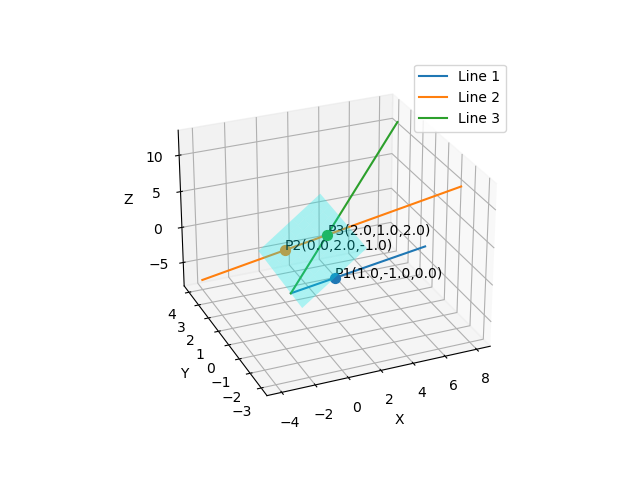
\includegraphics[width=0.5\columnwidth]{figs/fig1.png}
    \caption{}
    \label{fig:placeholder}
\end{figure}






\end{document}